\documentclass[fontsize=12pt, paper=a4, headinclude, twoside=false, parskip=half+, pagesize=auto, numbers=noenddot, open=right, toc=listof, toc=bibliography]{scrreprt}

%\usepackage[inner=4cm,outer=2cm]{geometry}
%\setlength{\oddsidemargin}{15,5pt}
%\setlength{\evensidemargin}{15,5pt}


%parskip:
  % full - Absätze haben großen Abstand
  % half - Absätze haben kleinen Abstand
  % off - Absätze haben Einzug (default)

% Bessere Unterstützung für PDF-Features
\usepackage[breaklinks=true]{hyperref}

%Schönere Schriftart laden
%\usepackage[latin1]{inputenc}
\usepackage[T1]{fontenc} % Ligaturen, richtige Umlaute im PDF
\usepackage[utf8]{inputenc}% UTF8-Kodierung für Umlaute usw
\usepackage[english]{babel} % Deutsche Silbentrennung verwenden
\usepackage{lmodern}
\renewcommand*\familydefault{\sfdefault}  %Zusatz für serifenlose Schrift.

%Zeilenabstand
\usepackage{setspace} % Zeilenabstand
\onehalfspacing % 1,5 Zeilen

% Schriften-Größen
\setkomafont{chapter}{\Huge\rmfamily} % Überschrift der Ebene
\setkomafont{section}{\Large\rmfamily}
\setkomafont{subsection}{\large\rmfamily}
\setkomafont{subsubsection}{\large\rmfamily}
\setkomafont{chapterentry}{\large\rmfamily} % Überschrift der Ebene in Inhaltsverzeichnis
\setkomafont{descriptionlabel}{\bfseries\rmfamily} % für description Umgebungen
\setkomafont{captionlabel}{\small\bfseries}
\setkomafont{caption}{\small}



% Einfachere Verwendung von korrekten Anführungszeichen
\usepackage[german=guillemets]{csquotes}
% oder german=quotes
% oder english=british oder english=american

%Mathematisches
\usepackage{amssymb}
\usepackage{amsmath}
\usepackage{amsthm}

%Quelltext einbinden
\usepackage{algorithm}
\usepackage{algorithmic}

%Abbildungen
\usepackage{graphicx}
\usepackage{caption}
\usepackage{subcaption}
\usepackage[verbose]{wrapfig}
\usepackage{float}
%\restylefloat{figure} %kannst du einen weiteren Positionierungsparameter [H] definieren. der setzt dir das bild an genau die stelle, wo du es haben willst. Ist allerdings auch nicht immer so praktisch.
% wenn du ein \pagebreak einfügst, gibt er dir vor der neuen seite noch alle gleitobjekte aus, die noch anstehen

%Zeichnen mit Tikz
\usepackage{tikz}
\usetikzlibrary{intersections,positioning,shapes.geometric,calc}

% Tabellen
\usepackage{multirow} % Tabellen-Zellen über mehrere Zeilen
\usepackage{multicol} % mehre Spalten auf eine Seite
\usepackage{tabularx} % Für Tabellen mit vorgegeben Größen
\usepackage{longtable} % Tabellen über mehrere Seiten
\usepackage{array}

%Bibliographie
\usepackage[square, comma, numbers, sort&compress, round]{natbib}
\usepackage{bibgerm} % Umlaute in BibTeX

%Umbenennung der vordefinierten definition- und example-Umgebung
\theoremstyle{definition}
\newtheorem{lecture}{Lecture}
\newtheorem{definition}{Definition}
\newtheorem{example}{Example}
\newtheorem{lemma}{Lemma}

% \newtheorem{theorem}{Satz}
% \newtheorem{constructing instructions}{Konstruktionsvorschrift}
% \newtheorem{properties}{Eigenschaften}
%\newtheorem{proposition}{Proposition}
%\newtheorem{korollar}{Corollary}
%\newtheorem{remark}{Remark}
%\newtheorem{consequences}{Consequences}
%\newtheorem{observation}{Observation}
%\newtheorem{conjecture}{Conjecture}
%\newtheorem{recall}{Recall}

\renewcommand{\labelenumi}{\roman{enumi})}

\renewcommand{\labelitemii}{$\bullet$}

\newcommand{\todo}[1]{
      {\colorbox{red}{ TODO: #1 }}
}
\newcommand{\todotext}[1]{
      {\color{red} TODO: #1} \normalfont
}

%bzgl `tocbasic` Warnung
\usepackage{scrhack}
 % Importiere die Einstellungen aus der Präambel
% hier beginnt der eigentliche Inhalt

\author{Lydia Buntrock}
\title{master thesis}
\date{August 2017}

\begin{document}
  % Titelseite
  \begin{titlepage}
    \pagestyle{empty}
  	
    	\vspace{20mm}
    	\begin{Large}
    	    \textbf{Origins and losses of parasitism}\\
          an analysis of the phylogenetic tree of life with a parsimony-like algorithm\\
    	\end{Large}

  	\clearpage
  \end{titlepage}

%---------------------------------------------------------------------------------------------------
%---------------------------------------------------------------------------------------------------
%--------------------------------------------------------------------------------------------------- 
\chapter*{Abstract}

\tableofcontents
\clearpage

%---------------------------------------------------------------------------------------------------
%---------------------------------------------------------------------------------------------------
%--------------------------------------------------------------------------------------------------- 
\chapter{Introduction}
  This paper is about the further development of parsimony algorithms for non-binary trees, applied 
  to the currently largest phylogeny synthesis tree of Open Tree Of Life, with the application to 
  the ancestral state reconstruction of parasitism. \\
  Researchers of the phylogenies have been dealt with the ancenstral state reconstruction in the 
  60s. The first methods were only brute force \todo{Quelle, siehe Fitch: Camin and Sokal 1965}. 
  Next came a set of parsimony algorithms such as: Fitch-parsimony \cite{Fitch1971}, 
  Wagner-parsimony \cite{Swofford1987} ... \todo{weitere?}. \\
  With more and more data, there is now the possibility to use more information to calculate the 
  probabilities of the ancestral states. In addition to the states of the leaves, algorithms could 
  also use branch lengths. The likelihood based algorithms came more in interest. \\
  Our focus came with another 'data extension'. We wanted to work with the biggest phylogenetic tree 
  that exists at this moment, which goes over all observed species. For most \todo{most?} species 
  there is no 
  phylogeny, but only a taxonomic classification. So the biggest 'phylogenetic tree' is a synthesis 
  of phylogenetic trees filled with a taxonomic tree given by Open Tree of Life \cite{Hinchliff2015}.
  This tree is not binary and therefore the developed algorithms are not directly applicable. \\
  In this work, we have looked at the algorithms that are generally suited to our data, to develop 
  them further for the not binary case, and finally to compare their usability with our sythesis 
  tree. \\
  We have decided to consider only parsimony algorithms since we have no information on branch 
  lengths and no other additional information like different transition probabilities of our states.

%---------------------------------------------------------------------------------------------------
%---------------------------------------------------------------------------------------------------
%--------------------------------------------------------------------------------------------------- 
\chapter{Methods}
  
  This work consist of two aspects. One is the application of the algorithm to our question

  Diese Arbeit besteht aus zwei Fragestellungen
  gute Algorithmen zu finden und sie auf unser Anwendungsbeispiel anzuwenden.

  Zur Bewertung der gefundenen / entwickelten algorithmen haben wir eine Simulation ausgeführt.

  Auf der Anderen Seite haben wir unser reales Problem aufgestellt, für die Algorithmen vorbereitet und 
  diese angewendet.
  

  Metadata -> Simulation ->  real Data

  %---------------------------------------------------------------------------------------------------
  %---------------------------------------------------------------------------------------------------
  \section{Metadata analysis}
    Properties of real Data - Metadata analysis

    There are some Parameters to find out or notice:
    \begin{itemize}
      \item transition probabilities of tags
      \item multifurcation
      \item nr of parasites to free-living
      \item nr of unknown nodes 
    \end{itemize}

  %---------------------------------------------------------------------------------------------------
  %---------------------------------------------------------------------------------------------------
  \section{Simulation}
    \begin{itemize}
      \item build random binary trees, tag these (parameters: parasites vs free-living, 
        beta-distribution)
      \item run fitch-parsimony, wagner-parsimony, our parsimony like algorithm
      \item build not binary tree (poisson distribution?)
      \item run new algorithms
      \item compare trees (distances)
    \end{itemize}

    \begin{enumerate}
      \item build random binary trees
      \item tag tree
      \item multifurcate tree
      \item run maximum parsimony algorithms
      \begin{itemize}
        \item Fitch
        \item Sankoff (Castor package)
        \item my algorithm
      \end{itemize}
      \item Evaluation
    \end{enumerate}

    %---------------------------------------------------------------------------------------------------
    \subsection{random binary tree}
      To get a random binary tree, I used the Phylo package from biopython. They offer a randomized
        function which returns a BaseTree \footnote{
          https://github.com/biopython/biopython/blob/master/Bio/Phylo/BaseTree.py
        }:
      \begin{lstlisting}
        from Bio import Phylo
        Phylo.BaseTree.Tree.randomized(number_leafnodes)
      \end{lstlisting}
      From the BaseTree class:
      \begin{lstlisting}
        def randomized(cls, taxa, branch_length=1.0, 
              branch_stdev=None):
        """Create a randomized bifurcating tree given a list
              of taxa.
          :param taxa: Either an integer specifying the number
              of taxa to create (automatically named taxon#), 
              or an iterable of taxon names, as strings.
          :returns: a tree of the same type as this class.
        """
      \end{lstlisting}
      \todo{Zitat von BaseTree und buildTree.py}

    %---------------------------------------------------------------------------------------------------
    \subsection{tag tree}
      At this point we want one fully tagged tree, and one less tagged tree which looks like our real 
        data.\\
      Let's say the first specie (the root node) was free-living (start with a parasite without a host 
        makes no sence). For every transition from a node to his child, we take a random number from
        the father distribution. We decided that from the biological perspective a beta distribution
        reflects our transition probabilities best (see Figure 2.1 \todo{ref einfügen}). \\
        For example when our father node was free-living, then we take from the free-living beta
        distribution. Is the number under the threshold for beeing parasite, we get a change and tag
        the current node as parasite. Otherwise we tag it as free-living. \\
        With this procedure we traverse through the tree from the root to every leave node. A part of
        this code you see here:
      \begin{lstlisting}
        from numpy import random
        if father_tag == 0:
          # freeliving_distribution:
          new_random = random.beta(a=A_FL, b=B_FL)
        else:
          # parasite_distribution:
          new_random = random.beta(a=A_P, b=B_P)
        tag = 0         # -> FL
        if new_random < percentage_parasites:
          tag = 1       # -> P
      \end{lstlisting}
      \begin{figure}
        \caption{60\% Free-living - 40\% Parasites}
        \centering
          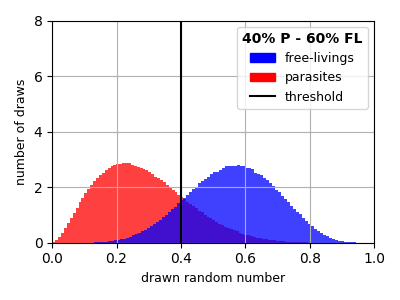
\includegraphics[width=0.5\textwidth]{Figures/40-60.png}
      \end{figure}
      \todo{Bessere Beschriftung, Plot neu erstellen! U.a. mit threshold}

      unknowns.. forget information.. nodelist

    %---------------------------------------------------------------------------------------------------
    \subsection{multifurcate tree}
  %---------------------------------------------------------------------------------------------------
  %---------------------------------------------------------------------------------------------------
  \section{real data analysis}
    \begin{itemize}
      \item Import tree
      \item Import interactions
      \item run castor algorithm / and others?
      \item interprete results (leave one out)
    \end{itemize}

  %---------------------------------------------------------------------------------------------------
  %---------------------------------------------------------------------------------------------------
  \section{Implementation}

%---------------------------------------------------------------------------------------------------
%---------------------------------------------------------------------------------------------------
%---------------------------------------------------------------------------------------------------
\chapter{Results}

%---------------------------------------------------------------------------------------------------
%---------------------------------------------------------------------------------------------------
%---------------------------------------------------------------------------------------------------
\chapter{Discussion}
  Wie gut ist der randomisiert erstellte Baum? \\
  Wie gut kommt unsere Simulation an die echte Datenlage heran. \\
  Fehlerqoute der Daten an sich? \\
  Wie gut ist unsere Datenlage? 3 mio knoten, 1.8 named species (leaf nodes), 200.000 leaf nodes mit 
  Information. \\
  Simulation von subtrees \\
  Welche Teile des Baumes sind gut, an welchen muss noch viel geforscht werden. \\
  Wieviele Origins haben wir gefunden, was bedeutet diese Zahl? \\
  
  Parameter der Simulation:
  \begin{itemize}
    \item Wie ist die Verteilung der vergessenen internen Knoten? Zum Wurzelknoten hin mehr vergessen?
    \item Wie sehen die übergangswahrscheinlichkeiten aus von P->FL und andersherum?
    \item Verteilung Parasiten zu Freilebend zu keine Information
  \end{itemize}


  Selecting of the 'right'  / best Distribution
  
%---------------------------------------------------------------------------------------------------
%---------------------------------------------------------------------------------------------------
%---------------------------------------------------------------------------------------------------
\bibliography{bibliographie}
\bibliographystyle{alphadin}


\end{document}
